In the implementation of our solution we have defined our own data
structure on which we execute the Tutte algorithm. We have
implemented some mechanisms to convert a tulip format graph to our own
graph structure and also to get information from our structure to insert them 
into a Tulip graph. In other words, our structure is a
temporary structure for storing information about nodes in order to
execute the Tutte algorithm.

\subsection{Issues}
As the Tulip data structure contains a lot of information, it is
expensive to manipulate them. Furthermore, we do not need all the
information from a given Tulip graph. For
instance, for a given node, we just want to know if it is fixed. For a
fixed node, position never changes during the Tutte algorithm. In
addition to that, as we are looking for performance, we need a light
structure matching the principe of Tutte algorithm. The following
points are the main reasons which lead us to set up a new data
structure.
\begin{enumerate}
\item The fact that a given node is fixed or not is indicated firstly
  by a mobility property. However, there is another property indicating
  nodes which are part of graph contouring, and these nodes need to be
  fixed too. Therefore, to deal with the fact that a given node is fixed or
  not, we need to manipulate two properties that cost a lot.

\item In Tulip data structure there is a hierarchy of graphs. However, we only need
  the parent of the graph. We do not need the sub-graph relation between graphs.

%%, the one which is not subgraph of another
  %%one
%% \item The informations about nodes are not in node but there is a
%% map between nodes and properties. For a given node, it cost a lot
%% to acces to one of its properties.

\end{enumerate}  

\subsection{Implementations}
We tested three implementations in order to find out the right one. Because we care of memory and speed, we merely store only the information needed to run the algorithm in our structure.

\subsubsection{First implementation}
In this implementation, our structure is constructed so that a given node
contains its neighbourhood. So one can easily access the neighbourhood
of a given node because it is very crucial in a Tutte algorithm
implementation. To do this, we define a class that contains the various
data needed on a given node (the attributes) and all the operations we
need to run on a node (the methods).

\newpage
\begin{lstlisting}
class MyNode {
 private:
  node n;
  bool mobile;
  Coord coord;  
  vector<MyNode *> voisin;

 public:
  MyNode();
  MyNode(const node n, const Coord coord);
  MyNode(const node n, const bool mob, const Coord coord);
  ~MyNode();
  
  const node getNode() const;
  bool getMobile() const;
  void setMobile(const bool b);
  const Coord getCoord() const;
  void setCoord(const Coord &);
  vector<MyNode *> * getVoisin();
  vector<MyNode *> getVoisin() const;
};
\end{lstlisting}
\noindent
\underline{\bf Vertex attributes needed}
\begin{dinglist}{70}
\item[n]: \texttt{node} type of \textsf{Tulip} library; contains the \texttt{ID} of the node.  
\item[mobile]: \texttt{boolean} type; is used to know a given node is considered fixed.
\item[coord]: \texttt{Coord} type of \textsf{Tulip} library; is used to store the node coordinates. 
\item[voisin]: \texttt{vector} type of \texttt{C++} library; contains the neighbourhood.
\end{dinglist}
\noindent
\underline{\bf Operations on a vertex}~\\
We used two types of operations or methods: \textsf{setter} and
\textsf{getter}. A \textsf{setter} is a method used to set the value of an
attribut and a \textsf{getter} is used to get the value of an attribut. For
a given attribut \texttt{attribut} , the corresponding setter and getter
are respectively \verb+setAttribut(args)+ and \verb+getAttribut()+. Below
are the lists of the setters and getters of nodes in our structure:
\begin{dinglist}{70}
\item[Setters]: \verb+getMobile(), getCoord(), getVoisin()+  
\item[Getters]: \verb+setMobile(const bool b), setCoord(const Coord &), getVoisin()+.
\end{dinglist}

\subsubsection{Second implementation}
In the second implementation, the built data structure aims to decrease
the number of pointer translation of the system. Also, the method to fill
our data structure tries to put the neighbourghood coordinates of a node 
near to its own.

A new basic class of MyNode\_ver2 have been implemented. The vector \\
\verb+vector<MyNode *> voisin+ is substituted by an integer \verb+index_neighbourhood+.

Here is the statement of this class:

\newpage
\begin{lstlisting}
  class MyNode_ver2 {
    public:
    node n;
    bool mobile;
    int index_neighbourhood;
    int degree;
  };
\end{lstlisting}

To store all the nodes, the neighboughoods and the coordinates, three tables are needed. 

\begin{lstlisting}
  vector<MyNode_ver2> MyNodes_2;
  vector<int> Neighbourhoods;
  vector<Vec2f> * coords;
\end{lstlisting}

\begin{dinglist}{70}
\item[MyNodes\_2]: contains all the nodes.
\item[Neighbourhoods]: contains the index of all the neighbourhoods.
\item[coords]: is used to store the nodes coordinates. 
\end{dinglist}

The attribute \verb+index_neighbourhood+ of the class \verb+MyNode_ver2+
gives the index of the neighbourhood of the node in the vector \verb+Neighbourhoods+.

\subsubsection{Third implementation}
In this third implementation, we do not use a class to store the
various data about node to run Tutte algorithm. 
As we are looking for a lighter data structure in order to ameliorate 
memory access, we use a \textsf{struct} to group data needed about a given node
under one name (\textsf{Data}). 
\begin{lstlisting}
  struct Data {
    node n;
    Coord coord;
    bool mobile;
  } Data;
\end{lstlisting}
In addition of the structure above, we use two tables: a \texttt{data store table} table to store data about nodes and \texttt{neighbourhoods table} to link nodes with their neighbourhoods. The picture below illustrate the principle.
\begin {figure}[H]
  \centering
  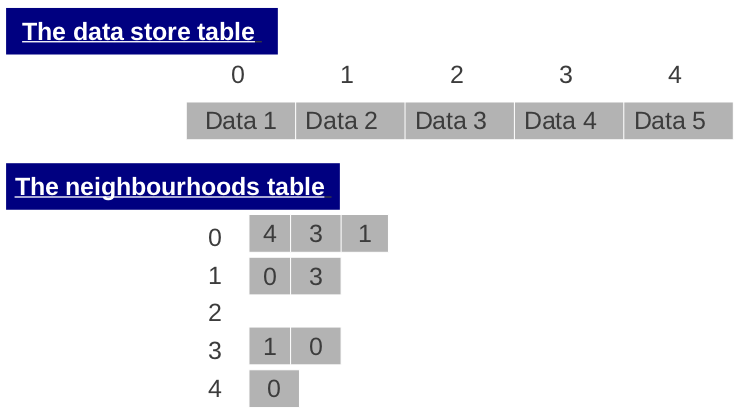
\includegraphics[scale=0.5]{img/struct3.png}
  \caption{Third implementation graph representation}
  \label{struct3}
\end {figure}
\noindent One can read in the \texttt{neighbourhoods table} that neighbours of the node 0 are nodes \texttt{4, 3,  1} and node 2 does not have neighbours. One can access all information about node 0 located at the index 0 of the \texttt{data store table}.  
%\subsection{Enhanced implementation}
